\documentclass[12pt,a4paper]{article}
\usepackage{mathtools}
\usepackage{parskip}
\usepackage[colorlinks=true, urlcolor=blue]{hyperref}
\usepackage{amsmath}
\usepackage{amssymb}
\usepackage{float}
\usepackage{fontenc}
\usepackage{graphicx}
\usepackage{caption}
\usepackage{subcaption}
\usepackage{multirow}

\renewcommand\thesubsection{\thesection.\arabic{subsection}}
\renewcommand\thesubsubsection{\thesubsection.\alph{subsubsection}}

\newcommand{\tab}{\hspace*{2em}}

\title{ADNI Progress report}
\author{Devendra Goyal\\Uniqname: devendra}

\date{\today}

\begin{document}
\maketitle

\part{Using HMMs to predict disease progression}

\section{Statistics about the data}
\label{sec:data}

There are several choices here for the dataset to be used:

\begin{itemize}
\item One of MRI/PET/CSF only
\item Some combination of 2/3 available modalities
\item Use all three modalities
\item Add demographics data to any of the above options
\end{itemize}

\emph{For now}, I have decided to use only the FDG-PET data for the
HMM problem. 

The pros are:

\begin{itemize}
\item The PET data is the cleanest and most easy dataset to process.
\item The feature space is relatively low dimensional. It is
  the \[mean, median, mode, min, max, stdev\] of the glucose
  expression for 5 expert defined regions in the brain - making it a
  total of 30 features for each patient.
\item Don't have to deal with failed segmentation amongst patients, or
  missing variables.
\item The pre-processing for PET scans accross all ADNI cohorts
  (ADNI1, ADNIGO, ADNI2) was done in one go by the same group using
  the same software, guaranteeing us homogenity in the data.
\end{itemize}

The cons are:

\begin{itemize}
\item Throwing away a lot of useful information from MRIs, CSFs, demographics
\item A small number of patients ($\approx 502$) have PET scans, which
  could making learning the HMM a problem
\end{itemize}

Some possible solutions for the future:

\begin{itemize}
\item It is potentially a very interesting problem to think about the
  use of observations from multiple modalities in a HMM setting. The
  reason this is better than doing it in an SVM setting is - due to
  the generative nature of the HMMs, we do not have to throw away
  patients who have missing observations for any of the three modalities.
\item For the same reason as above, it will be interesting to think
  about the problem of dealing with missing data.
\end{itemize}

\part{Establishing the baseline}

\section{Statistics about the Data}
\label{sec:stats}

The results shown in this document are based on the ADNI-1
cohort. There are several pros and cons of this decision:

\subsection{Pros}

\begin{itemize}
\item All the pre-processed features uploaded on the ADNI website
  operate on the entire cohort, thus there is homogeneity in terms of
  the features available for each patient across each modailty. MRI
  images for ADNI-GO/2 have been processed using different versions of
  the same software, and are also collected using a higher resolution
  MRI machine. While this is not a dealbreaker per se, it will require
  significantly more work to process all the images using the same
  software and generate similar features.
\item Most of the recent literature (~5 years) relies on data from ADNI1
  only to report results. This will give us a chance to compare our
  results directly with some of these reported results.
\item ADNI-1 is the best dataset to track patients longitudinally, as
  it was started in $2004$ and we have about $8$ years' worth of data
  for all MCI and AD patients that the protocol chose to follow (more
  on this later). 
\end{itemize}

\subsection{Cons}

\begin{itemize}
\item ADNI1 has CSF data available for only about 20\% of the
  patients. This number will become even smaller when we look at the
  number of patients that have data available for all 3 modalities.
\end{itemize}

Below is a chart summarizing the study design:

\begin{figure}[ht]
  \centering
  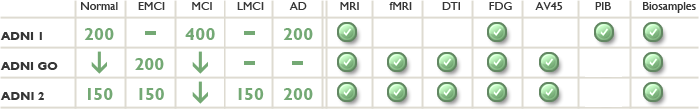
\includegraphics[width=\textwidth]{study-design.png}
  \caption{\label{fig:design}ADNI study design}
\end{figure}

The table below summarizes the number for the \textbf{ADNI1} cohort
only, for the MRI and PET modalities.

\begin{tabular}[H]{c | c | c | c | c | c}
  & NL & \multicolumn{3}{|c|}{MCI} & AD\\
\hline
& & MCI-c & MCI-nc & MCI-rev &\\
\hline
FDG-PET & 102 & 94 & 96 & 13 & 97\\
MRI(clean) & 180 & 133 & 132 & 10 & 123\\
MRI(complete) & 229 & 196 & 183 & 18 & 192\\
FDG+MRI(clean) & 79 & 66 & 68 & 9 & 62\\
FDG+MRI(complete) & 102 & 94 & 96 & 13 & 97\\
\end{tabular}

\section{SVMs on classification task}
\label{sec:svm}

\subsection{NL vs AD}
\label{sec:nl-vs-ad}

\subsubsection{MRI}
\label{sec:mri}

\begin{figure}[H]
  \centering
  \includegraphics[width=\textwidth]{nl-ad/mri-coarse-accuracy.png}
  \caption{\label{figaa:design}Hyperparameter search for MRI images
    optimizing for classification accuracy}
\end{figure}

\begin{figure}[H]
  \centering
  \includegraphics[width=\textwidth]{nl-ad/mri-coarse-auroc.png}
  \caption{\label{fig:dbbesign}Hyperparameter search for MRI images
    optimizing for AUROC}
\end{figure}

\begin{figure}[H]
  \centering
  \includegraphics[width=\textwidth]{nl-ad/mri-acc.png}
  \caption{\label{fig:desssign}Classification accuracy (test set) for MRI images}
\end{figure}

\begin{figure}[H]
  \centering
  \includegraphics[width=\textwidth]{nl-ad/mri-auroc.png}
  \caption{\label{fig:desigggn}AUROC for MRI images (test set)}
\end{figure}

\subsubsection{PET}
\label{sec:pet}

\begin{figure}[H]
  \centering
  \includegraphics[width=\textwidth]{nl-ad/pet-coarse-accuracy.png}
  \caption{\label{uufig:design}Hyperparameter search for PET images
    optimizing for classification accuracy}
\end{figure}

\begin{figure}[H]
  \centering
  \includegraphics[width=\textwidth]{nl-ad/pet-coarse-auroc.png}
  \caption{\label{fiqeg:design}Hyperparameter search for PET images
    optimizing for AUROC}
\end{figure}

\begin{figure}[H]
  \centering
  \includegraphics[width=\textwidth]{nl-ad/pet-acc.png}
  \caption{\label{fig:fsdhvdesign}Classification accuracy (test set) for PET images}
\end{figure}

\begin{figure}[H]
  \centering
  \includegraphics[width=\textwidth]{nl-ad/pet-auroc.png}
  \caption{\label{fig:design}AUROC for PET images (test set)}
\end{figure}

\subsubsection{CONCAT}
\label{sec:cat}

\begin{figure}[H]
  \centering
  \includegraphics[width=\textwidth]{nl-ad/concat-acc.png}
  \caption{\label{fig:desigffhn}Classification accuracy (test set) for PET images}
\end{figure}

\subsection{NL vs MCI}

\subsubsection{MRI}

\begin{figure}[H]
  \centering
  \includegraphics[width=\textwidth]{nl-mci/mri-accuracy.png}
  \caption{\label{desigan}Classification accuracy (test set) for MRI images}
\end{figure}

\subsubsection{PET}

\begin{figure}[H]
  \centering
  \includegraphics[width=\textwidth]{nl-mci/pet-accuracy.png}
  \caption{\label{afig:design}Classification accuracy (test set) for MRI images}
\end{figure}

\subsubsection{CONCAT}

\begin{figure}[H]
  \centering
  \includegraphics[width=\textwidth]{nl-mci/concat-accuracy.png}
  \caption{\label{fffpig:design}Classification accuracy (test set) for MRI images}
\end{figure}

\end{document}